%
%  RULES OF THE GAME
%
%  * 80 characters
%  * line breaks at the ends of sentences
%  * Sun Solar Earth all capitalized when referring to our peeps, even as in
%    "extra-Solar"
%  * eqnarrys ONLY
%  * that is all.
%

\documentclass[12pt,preprint]{aastex}

\include{vc}

\usepackage{color,hyperref}
\definecolor{linkcolor}{rgb}{0,0,0.5}
\hypersetup{colorlinks=true,linkcolor=linkcolor,citecolor=linkcolor,
            filecolor=linkcolor,urlcolor=linkcolor}
\usepackage{url}
\usepackage{amssymb,amsmath}
\usepackage{subfigure}

\newcommand{\project}[1]{{\sffamily #1}}
\newcommand{\kepler}{\project{Kepler}}
\newcommand{\terra}{\project{TERRA}}
\newcommand{\license}{MIT License}

\newcommand{\paper}{\textsl{Article}}

\newcommand{\foreign}[1]{\emph{#1}}
\newcommand{\etal}{\foreign{et\,al.}}
\newcommand{\etc}{\foreign{etc.}}
\newcommand{\True}{\foreign{True}}
\newcommand{\Truth}{\foreign{Truth}}

\newcommand{\figref}[1]{\ref{fig:#1}}
\newcommand{\Fig}[1]{Figure~\figref{#1}}
\newcommand{\fig}[1]{\Fig{#1}}
\newcommand{\figlabel}[1]{\label{fig:#1}}
\newcommand{\Tab}[1]{Table~\ref{tab:#1}}
\newcommand{\tab}[1]{\Tab{#1}}
\newcommand{\tablabel}[1]{\label{tab:#1}}
\newcommand{\Eq}[1]{Equation~(\ref{eq:#1})}
\newcommand{\eq}[1]{\Eq{#1}}
\newcommand{\eqalt}[1]{Equation~\ref{eq:#1}}
\newcommand{\eqlabel}[1]{\label{eq:#1}}
\newcommand{\Sect}[1]{Section~\ref{sect:#1}}
\newcommand{\sect}[1]{\Sect{#1}}
\newcommand{\App}[1]{Appendix~\ref{sect:#1}}
\newcommand{\app}[1]{\App{#1}}
\newcommand{\sectlabel}[1]{\label{sect:#1}}

\newcommand{\dd}{\ensuremath{\,\mathrm{d}}}
\newcommand{\bvec}[1]{\ensuremath{\boldsymbol{#1}}}
\newcommand{\appropto}{\mathrel{\vcenter{
  \offinterlineskip\halign{\hfil$##$\cr
    \propto\cr\noalign{\kern2pt}\sim\cr\noalign{\kern-2pt}}}}}
\newcommand{\densityunit}{{\ensuremath{\mathrm{nat}^{-2}}}}

% TO DOS
\newcommand{\todo}[3]{{\color{#2} \emph{#1} TODO: #3}}
\newcommand{\dfmtodo}[1]{\todo{DFM}{red}{#1}}
\newcommand{\hoggtodo}[1]{\todo{HOGG}{blue}{#1}}
\newcommand{\mortontodo}[1]{\todo{MORTON}{green}{#1}}

% Document specific variables.
\newcommand{\rate}{\ensuremath{\Gamma}}
\newcommand{\ratepar}{{\ensuremath{\theta}}}
\newcommand{\ratepars}{{\ensuremath{\bvec{\ratepar}}}}
\newcommand{\obs}[1]{\ensuremath{\hat{#1}}}
\newcommand{\radius}{\ensuremath{R}}
\newcommand{\period}{\ensuremath{P}}
\newcommand{\completeness}{{\ensuremath{Q_\mathrm{c}}}}
\newcommand{\transitprob}{{\ensuremath{Q_\mathrm{t}}}}
\newcommand{\data}{{\ensuremath{\bvec{x}}}}
\newcommand{\entry}{{\ensuremath{\bvec{w}}}}
\newcommand{\catalog}{{\ensuremath{\bvec{\entry}}}}

\newcommand{\interim}{{\ensuremath{\bvec{\alpha}}}}

\newcommand{\binarea}{{\ensuremath{\Delta}}}
\newcommand{\bincenter}{{\ensuremath{\bvec{x}}}}
\newcommand{\binheight}{{\ensuremath{w}}}
\newcommand{\binheights}{{\ensuremath{\bvec{\binheight}}}}

\newcommand{\mean}{{\ensuremath{\mu}}}
\newcommand{\smooth}{{\ensuremath{\lambda}}}
\newcommand{\smoothpars}{{\ensuremath{\bvec{\smooth}}}}
\newcommand{\cov}{{\ensuremath{\mathrm{K}}}}

\newcommand{\modela}{\emph{Catalog A}}
\newcommand{\modelb}{\emph{Catalog B}}

\newcommand{\gammaearth}{{\ensuremath{\rate_\oplus}}}

\begin{document}

\title{%
    Exoplanet population inference and the rate of Earth analogs \\
    from noisy, incomplete catalogs
}

\newcommand{\nyu}{2}
\newcommand{\mpia}{3}
\newcommand{\cds}{4}
\newcommand{\princeton}{5}
\newcommand{\berkeley}{6}
\author{%
    Daniel~Foreman-Mackey\altaffilmark{1,\nyu},
    David~W.~Hogg\altaffilmark{\nyu,\mpia,\cds},
    Timothy~D.~Morton\altaffilmark{\princeton}
}
\altaffiltext{1}         {To whom correspondence should be addressed:
                          \url{danfm@nyu.edu}}
\altaffiltext{\nyu}      {Center for Cosmology and Particle Physics,
                          Department of Physics, New York University,
                          4 Washington Place, New York, NY, 10003, USA}
\altaffiltext{\mpia}     {Max-Planck-Institut f\"ur Astronomie,
                          K\"onigstuhl 17, D-69117 Heidelberg, Germany}
\altaffiltext{\cds}      {Center for Data Science,
                          New York University,
                          4 Washington Place, New York, NY, 10003, USA}
\altaffiltext{\princeton}{Department of Astrophysics, Princeton University,
                          Princeton, NJ, 08544, USA}

\begin{abstract}

Many exoplanets have been discovered and characterized; it is now possible to
study the population as a whole.
Although no true extra-Solar Earth analog is known, hundreds of planets have
been found around Sun-like stars that are either Earth-sized but on shorter
periods, or else on year-long orbits but somewhat larger.
Under strong assumptions, these exoplanet catalogs have been used to make an
extrapolated estimate of the rate at which Sun-like stars host Earth analogs.
These studies are complicated by the fact that every catalog is censored by
non-trivial selection effects and detection efficiencies, and every property
(period, radius, \etc) is measured noisily.
Here we present a general hierarchical probabilistic framework for making
justified inferences about the population of exoplanets, taking into account
survey completeness and, for the first time, \emph{observational
uncertainties}.
We are able to make fewer assumptions about the distribution than previous
studies; we only require that the occurrence rate density be a smooth function
of period and radius (employing a Gaussian process).
By applying our method to synthetic catalogs, we demonstrate that it produces
more accurate estimates of the whole population than standard procedures based
on weighting by inverse detection efficiency.
We apply the method to an existing catalog of small planet candidates around G
dwarf stars (Petigura \etal\ 2013).
We confirm a previous result that the radius distribution changes slope near
Earth radius.
We find that the rate density of Earth analogs is about 0.02 (per star per
natural logarithmic bin in period and radius) with large uncertainty.
This number is much smaller than previous estimates made with the same data
but stronger assumptions.

\end{abstract}

\keywords{%
methods: data analysis
---
methods: statistical
---
catalogs
---
planetary systems
---
stars: statistics
}

\section{Introduction}

NASA's \kepler\ mission has enabled the discovery of thousands of exoplanet
candidates (\citealt{kepler-catalog}).
While many of these candidates have not been confirmed as bona fide planets,
there is evidence that the false positive rate is low (\citealt{morton,
fressin-fp}), enabling conclusions about the population of planets based on
the catalog of candidates.
Many of these planets orbit Sun-like stars (\citealt{petigura}), where the
definition of Sun-like is given in terms of the star's temperature and surface
gravity.
Given these catalogs, it is interesting to ask what we can say about the
population of exoplanets as a function of their physical parameters
(period, radius, \etc).
Observational constraints on the population can inform theories of planet
formation (\dfmtodo{CITE}) and place probabilistic bounds on the abundance of
Earth analogs\footnote{For our purposes, an ``Earth analog'' is an Earth-sized
exoplanet orbiting a Sun-like star with a year-long period.}.

\citet{petigura} recently published constraints on this function based on
their independent analysis of the \kepler\ light curves for 42,000 Sun-like
stars.
This study was especially novel because the authors developed an independent
planet search pipeline (\terra; \citealt{petigura-a}) and determined the
detection efficiency of their analysis empirically by injecting synthetic
signals into real light curves measured by \kepler.
The occurrence rate function determined by \citet{petigura} agreed
qualitatively with previous studies of small planets orbiting Sun-like stars
(\citealt{dong}).
In particular, both papers describe a ``flattening'' rate function (in
logarithmic radius) for planets around Earth's radius.
Even though no Earth analogs were discovered in their search, \citet{petigura}
used the small candidates that the did find to place an extrapolated
constraint on the frequency of Earth-like exoplanets, assuming a flat
occurrence rate density in logarithmic period.

A very important component of any study of exoplanet populations is the
treatment of detection efficiency.
Speaking qualitatively, in a transit survey, small planets with long periods
are much harder to detect than large planets orbiting close to their star.
This effect is degenerate with any inferences about the rate density and it
can be hard to constraint quantitatively.
In practice, there are three methods for taking this effect into account:
\emph{(a)} making conservative cuts on the candidates and assuming that the
resulting catalog is complete (\citealt{catanzarite, traub, tremaine}),
\emph{(b)} asserting an analytic form for the detection efficiency as a
function of approximate signal-to-noise (\citealt{youdin, howard, dressing,
dong, fressin-fp, morton-swift}), and \emph{(c)} determining the detection
efficiency empirically by injecting synthetic signals into the raw data and
testing recovery (\citealt{petigura-a, petigura}).

There are two pedagogically different methods that are commonly used to infer
the occurrence rate density from a catalog and a detection efficiency
specification.
The first is an intuitive method that we will refer to as
inverse-detection-efficiency procedure and the second is based on the
likelihood function of the catalog given a parametric rate density.
The inverse-detection-efficiency method involves making a histogram of the
objects in the catalog where each point is weighted by its inverse detection
probability.
This method is very popular in the literature (\citealt{howard, dong,
dressing, swift, petigura}) even though it is not motivated probabilistically.
The alternative ``likelihood'' method models the catalog as a Poisson
realization of the \emph{observable} rate density of exoplanets taking the
survey detection efficiencies and transit probabilities into account.
This technique has been used to constrain parametric models---a broken power
law, for example---for the occurrence rate density (\citealt{tabachnik,
youdin, dong}).
There are many reasons to prefer a result based on an optimization of a
likelihood function and as we show in \sect{model}, if we model the occurrence
rate density as a piecewise constant function, the
inverse-detection-efficiency method can be derived as a special case of the
likelihood method with a specific set of assumptions.

In every previous study of exoplanet occurrence rates, the authors have
assumed that the measurement uncertainties are negligible.
This assumption is not justified because these uncertainties---especially on
measurements (like exoplanet radius) that depend on the stellar
parameters---can be large compared to the scales of interest.
In this \paper, we develop a flexible framework for probabilistic inference of
exoplanet occurrence rate density that can be applied to incomplete catalogs
with \emph{non-negligible observational uncertainties}.
We generalize the inference method introduced by \citet{hogge} to account for
survey detection efficiencies.
We run tests on simulated datasets---comparing results with the standard
techniques that neglect observational uncertainties---and apply our method to
a real catalog of small planets transiting Sun-like stars
(\citealt{petigura}).

For the purposes of this \paper, we make some strong assumptions, although we
argue that they are weaker than the implicit assumptions in previous
studies.
None of these assumptions is necessary for the validity of our general method
but they do simplify the specific procedures we employ.
Specifically, we assume that
\begin{itemize}

\item the candidates in the catalog are independent draws from an
inhomogeneous Poisson process set by the censored occurrence rate density,

\item every candidate is a real exoplanet (there are no false positives),

\item the observational uncertainties on the physical parameters are
non-negligible but known (the catalog provides probabilistic constraints on
the parameters),

\item the detection efficiency of the pipeline is known, and

\item the \True\footnote{In this \paper, we use ``\True'' to describe an
observable (for example, the exoplanet occurrence rate density) that would be
trivially measured in the limit of very high signal-to-noise data.
We use ``true'' to describe a simulation quantity with a value exactly known
to us.} occurrence rate density is \emph{smooth}\footnote{We give our
definition of ``smooth'' in more detail below but our model is very flexible
so this is not a strong restriction.}.

\end{itemize}
The first assumption---conditional independence of the candidates---is
reasonable since the dataset that we consider explicitly includes only single
transiting systems (\citealt{petigura}).
This is a limitation of the input catalog.
When considering other datasets it will be interesting and important to take
multiple transiting systems into account (\citealt{lissauer, tremaine, fang})
and this would be possible using a conditional distributions (as developed by
\citealt{tremaine}).
The second assumption---neglecting false positives---is also strong and only
weakly justified by estimates of low false positive rates in the \kepler\ data
(\citealt{fressin-fp, morton}).
For this \paper, we will neglect this issue and only comment on the effects
but the prior distributions published by \citet{fressin-fp} would be directly
applicable in our method and this would be a very interesting generalization.

We must emphasize one very important consequence of our assumptions.
We assume that the catalog of exoplanet candidates is only missing planets
with probabilities given by the empirical detection efficiency.
In detail this must be false; the detection efficiency we use
doesn't take into account the fact that the catalog doesn't include multiple
transiting systems.
A large fraction of the transiting planets discovered by the \kepler\ transit
search pipeline are members of multiple transiting systems (see
\citealt{lissauer}, for example).
Since \citet{petigura} only detected at most one planet per system, their
catalog is actually a list of planet candidates \emph{without a more
detectable companion}.
The global effects of this selection is not trivial and an in-depth discussion
is beyond the scope of this \paper\ but all of the results should be
interpreted with this caveat in mind.

Conditioned on our assumptions and the choices made in planet detection,
vetting and characterization pipeline (\citealt{petigura-a, petigura}), we
constrain the rate density of small exoplanets orbiting Sun-like stars.
As part of this analysis we also place probabilistic constraints on the rate
density\footnote{In this \paper, we use the word ``rate'' to indicate the
dimensionless expectation value of a Poisson process and the words ``rate
density'' to indicate a quantity that must be integrated over a finite bin in
period and radius to deliver a rate.} of Earth analogs \gammaearth\ which we
define as \emph{the expected number of planets per star per natural
logarithmic bin in period and radius, evaluated at the period and radius of
Earth}
% A certain distinguished prof at the IAS owes us beer.
\begin{eqnarray}
\gammaearth &=&
\left.\frac{\dd N}{\dd\ln\period\,\dd\ln\radius}\right|
_{\radius=\radius_\oplus,\,\period=\period_\oplus}\quad.
\end{eqnarray}
Since no Earth analogs have been detected, this constraint requires an
extrapolation in both period and radius.
\citet{petigura} performed this extrapolation by assuming that the period
distribution of planets in a small bin in radius is flat, obtaining
$\gammaearth \approx 0.12$.
We relax this assumption and extrapolate only by assuming that the occurrence
rate density is a smooth function of period and radius; we find a much lower
value for \gammaearth.
We enforce the smoothness constraint by applying a flexible Gaussian process
regularization to the bin heights.

In the next Section, we introduce the concept of hierarchical inference, how
it applies to the problem at hand, and we derive the importance sampling
approximation to the marginalized likelihood (this is a generalization of the
method from \citealt{hogge}).
Then, in \sect{model}, we describe how to include detection efficiencies in
this model and derive a probabilistic motivation for the standard
inverse-detection-efficiency weighting procedure.
After testing our method on synthetic catalogs in \sect{valid}, we use the
catalog of planet candidates and the empirically determined detection
efficiency from \citet{petigura} to measure the occurrence rate density of
Earth analogs.

\section{A brief introduction to hierarchical inference}

In this \paper, we are asking the question: \emph{what constraints can we put
on the occurrence rate density of exoplanets given all the light curves
measured by \kepler?}
Throughout this \paper, we use the notation $\rate_\ratepars(\entry)$ for the
occurrence rate density \rate---parameterized by the parameters \ratepars---as
a function of the physical parameters \entry\ (orbital period, planetary
radius, \etc).
In this framework, the occurrence rate density can be ``parametric''---for
example, a power law---or a ``non-parametric'' function---such as a histogram
where the bin heights are the parameters \ratepars.
The light curve for a particular target $k$ is called $\data_k$ and the
\True\ set of physical parameters for that same object are given by
$\entry_k$.
A catalog provides a set of constraints on the parameters $\{\entry_k\}$
conditioned on the set light curves $\{\data_k\}$.

Any inference about the rate density parameters can be formally addressed by
evaluating the \emph{marginalized likelihood function}
\begin{eqnarray}\eqlabel{crazylike}
p(\{\data_k\}\,|\,\ratepars) &=&
    \int p(\{\data_k\}\,|\,\{\entry_k\})
    \,p(\{\entry_k\}\,|\,\ratepars)
    \dd\{\entry_k\}
\end{eqnarray}
where, as we mentioned above, $\{\data_k\}$ is the set of all light curves,
one light curve $\data_k$ per target $k$, \ratepars\ is the vector of
parameters describing the population occurrence rate density
$\rate_\ratepars(\entry)$ and $\entry_k$ is the vector of physical parameters
describing the planetary system (orbital periods, radius ratios, stellar
radius, \etc) around target $k$.
In this equation, our only assumption is that the datasets depend on the
rate density of exoplanets only through the catalog $\{\entry_k\}$.
In our case, this assumption qualitatively means that the signals found in the
light curves depend only on the actual planet properties and not on the
distributions from which they are drawn.
It is worth emphasizing that---as we will discuss further below---the catalog
only provides \emph{probabilistic constraints} on $\{\entry_k\}$; not perfect
delta-function measurements.

In other words, a catalog is a dimensionality reduction of the raw data with
all the relevant information retained.
In the context of \kepler, the catalog reduces the set of downloaded pixel
time series (approximately 70,000 data points for the typical \kepler\ target)
to probabilistic constraints on a handful of physical parameters---\entry\
from above---like the orbital period and planetary radius.
If we take this set of parameters $\{\entry_k\}$ as \emph{sufficient
statistics} of the data then we can, in theory, compute \eq{crazylike}---up to
an unimportant constant---without ever looking at the raw data again.
This is permitted because the catalog provides constraints on the posterior
probability of the parameters $\{\entry_k\}$ under some choice of
\emph{interim prior} \interim
\begin{eqnarray}\eqlabel{crazypost}
p(\{\entry_k\}\,|\,\{\data_k\},\,\interim) &=&
\frac{p(\{\data_k\}\,|\,\{\entry_k\})\,p(\{\entry_k\}\,|\,\interim)}
     {p(\{\data_k\}\,|\,\interim)} \quad.
\end{eqnarray}
The interim prior $p(\{\entry_k\}\,|\,\interim)$ is the prior
function---parameterized by \interim---that the author of the catalog chose
when making their measurements.

It turns out that we can use these posterior measurements to simplify
\eq{crazylike} to a form that can, in many common cases, be evaluated
efficiently.
To find this result, multiply the integrand in \eq{crazylike} by
\begin{eqnarray}
\frac{p(\{\entry_k\}\,|\,\{\data_k\},\,\interim)}
     {p(\{\entry_k\}\,|\,\{\data_k\},\,\interim)}
\end{eqnarray}
and use \eq{crazypost} to find
\begin{eqnarray}\eqlabel{simplemarglike}
\frac{p(\{\data_k\}\,|\,\ratepars)}{p(\{\data_k\}\,|\,\interim)} &=&
    \int
    \frac{p(\{\entry_k\}\,|\,\ratepars)}{p(\{\entry_k\}\,|\,\interim)}\,
    p(\{\entry_k\}\,|\,\{\data_k\},\,\interim)
    \dd\{\entry_k\} \quad.
\end{eqnarray}
The data only enter this equation through the posterior constraints provided
by the catalog $\{\entry_k\}$!
For our purposes, this is the \emph{definition} of hierarchical inference.

The constraints in \eq{crazypost} can always be---and often are---propagated
as a list of $N$ samples $\{\entry_k^{(n)}\}$ from the posterior
\begin{eqnarray}
\{\entry_k\}^{(n)} &\sim& p(\{\entry_k\}\,|\,\{\data_k\},\,\interim) \quad.
\end{eqnarray}
We can use these samples to approximately compute the integral in
\eq{simplemarglike} as
\begin{eqnarray}\eqlabel{importance}
\frac{p(\{\data_k\}\,|\,\ratepars)}{p(\{\data_k\}\,|\,\interim)} &\approx&
    \frac{1}{N} \sum_{n=1}^N
    \frac{p(\{\entry_k^{(n)}\}\,|\,\ratepars)}
         {p(\{\entry_k^{(n)}\}\,|\,\interim)} \quad.
\end{eqnarray}
This is very efficient to compute as long as an evaluation of
$p(\{\entry_k^{(n)}\}\,|\,\ratepars)$ is not very expensive.
That being said, this could be a high variance estimator depending on the
initial choice of $p(\{\entry_k^{(n)}\}\,|\,\interim)$ but in our case, we'll
show that not many samples are needed to get an accurate estimate.
\Eq{importance} is the \emph{importance sampling approximation} to the
integral in \eq{simplemarglike} where the trial density is the posterior
probability for the catalog measurements.

A very simple example is the familiar procedure of making a histogram.
If you model the function $p(\{\entry_k\}\,|\,\ratepars)$ as a piecewise
constant rate density---where the bin heights are the parameters---and if the
uncertainties on the catalog are negligible compared to the bin widths then
the maximum marginalized likelihood solution for \ratepars\ is a histogram of
the catalog entries.
The case of non-negligible uncertainties is described by \citet{hogge} using a
method similar to the one discussed here.

\section{Model generalities}
\sectlabel{model}

In the inference procedure described above, we only discussed an abstract
occurrence rate density.
To make it more concrete, we'll model the catalog as a Poisson draw from the
\emph{observable} rate density $\obs{\rate}_\ratepars$.
This leads to the previously known result (see \citealt{tabachnik,youdin} for
some of the examples from the exoplanet literature)
\begin{eqnarray}\eqlabel{poisson-like}
p(\{\entry_k\}\,|\,\ratepars) &=&
    \exp\left(-\int \obs{\rate}_\ratepars (\entry) \dd\entry\right) \,
    \prod_{k=1}^K \obs{\rate}_\ratepars (\entry_k)\quad.
\end{eqnarray}
In this equation, the integral in the normalization term is the expected
number of observable exoplanets in the sample.
A further assumption that we have made in \eq{poisson-like} is that each
object is an independent sample from the inhomogeneous Poisson process set by
the rate density.
This assumption---though it is often made---cannot be correct when we consider
systems of multiple planets.
It is possible to relax this assumption (see \citealt{tremaine} for a related
technique) but this generalization is beyond the scope of the current \paper.

The main thing to note here is that $\obs{\rate}_\ratepars$ is the rate
density of exoplanets that you would expect to observe taking into account the
geometric transit probability and any other detection efficiencies.
In practice, we can model the observable rate density as
\begin{eqnarray}\eqlabel{obs-rate}
\obs{\rate}_\ratepars(\entry) &=&
    \completeness(\entry)\,\rate_\ratepars(\entry)
\end{eqnarray}
where $\completeness(\entry)$ is the detection efficiency (including transit
probability) at \entry\ and $\rate_\ratepars(\entry)$ is the object that we
want to infer: the \True\ occurrence rate density.
Up to this point, we haven't discussed any specific functional form for
$\rate_\ratepars(\entry)$ and all of this derivation is equally applicable
whether we model the rate density as (for example) a broken power law or
a histogram.

The observed rate density \obs{\rate} is a quantitative description of the
rate density at which planets appear in the \citet{petigura} catalog; it is
not a description of the \True\ rate density of exoplanets.
Inasmuch as the detection efficiency $\completeness(\entry)$ is calculated
correctly, the function $\rate_\ratepars(\entry)$ will represent the \True\
rate density of exoplanets, at least where there is support in the data.
In practice, an estimate of the detection efficiency will not include every
decision or effect in the pipeline.
One example in this case is that the completeness function does not account
for the explicit removal of second (and third, and so on) planets.
In principle a more complete description of the detection efficiency can be
included and as this function becomes more accurate, our inferences about the
\True\ rate density $\rate_\ratepars(\entry)$ will be less biased.

For the results in this \paper, we will assume that the completeness function
$\completeness(\entry)$ is known empirically but that is not a requirement for
the validity of this method.
Instead, we could use a functional form for it and infer the parameters
(\dfmtodo{cite all the papers that do the ramp, step function, whatever}).

Now, we can substitute \eq{poisson-like} into \eq{simplemarglike} and apply
the importance sampling approximation (\eqalt{importance}) to derive the
following expression for the marginalized likelihood
\begin{eqnarray}\eqlabel{money}
\frac{p(\{\data_k\}\,|\,\ratepars)}{p(\{\data_k\}\,|\,\interim)} &\approx&
    \exp\left(-\int \obs{\rate}_\ratepars (\entry) \dd\entry\right) \,
    \prod_{k=1}^K
    \frac{1}{N_k} \sum_{n=1}^{N_k}
    \frac{\obs{\rate}_\ratepars (\entry_k^{(n)})}
         {p(\entry_k^{(n)}\,|\,\interim)} \quad.
\end{eqnarray}
In this equation, we're making the further assumption that the catalog treated
the objects independently.
In other words, we have per-object posterior samples
\begin{eqnarray}
\entry_k^{(n)} &\sim& p(\entry_k\,|\,\data_k,\,\interim) \quad.
\end{eqnarray}
\Eq{money} is the \emph{money equation} for our method.
It lets us efficiently compute the \emph{marginalized likelihood of the entire
set of light curves for a particular occurrence rate density}.

\paragraph{Inverse-detection-efficiency}
It's now interesting to take a brief aside and discuss the connection between
our model and the commonly used inverse-detection-efficiency procedure
(\citealt{howard,dressing,petigura}).
This procedure involves making a weighted histogram of the catalog entries
where the weight for object $\entry_k$ is $1/\completeness(\entry_k)$.
This makes intuitive sense but the standard formulation does not have a clear
probabilistic justification or interpretation.
\hoggtodo{Find the papers that Tremaine suggested that we look at re:vmax and
discuss the motivation in those cases.}

If we model the occurrence rate density as a histogram with $J$ fixed bin
volumes $\binarea_j$
\begin{eqnarray}
\rate_\ratepars (\entry) &=& \left\{\begin{array}{ll}
\ratepar_1 & \entry \in \binarea_1,\\
\ratepar_2 & \entry \in \binarea_2,\\
\cdots \\
\ratepar_J & \entry \in \binarea_J,\\
0 & \mathrm{otherwise}
\end{array}\right.
\end{eqnarray}
then \eq{poisson-like} becomes
\begin{eqnarray}
\ln p(\{\entry_k\}\,|\,\ratepars) &=&
    \sum_{k=1}^K \sum_{j=1}^J \mathbf{1}[\entry_k \in
        \binarea_j]\,\ln\completeness(\entry_k)\,\ratepar_j
    -\sum_{j=1}^J\ratepar_j\,\int_{\binarea_j} \completeness(\entry)\dd\entry
\end{eqnarray}
where the indicator function $\mathbf{1}[\cdot]$ is one if $\cdot$ is true and
zero otherwise.
If we take the gradient of this function with respect to \ratepars\ and set it
equal to zero, we find the maximum likelihood result
\begin{eqnarray}\eqlabel{ml-ide}
{\ratepar_j}^* &=&
\frac{N_j}{\int_{\binarea_j} \completeness(\entry)\dd\entry}
\end{eqnarray}
where $N_j$ is the number of objects that fall within the bin $j$.
We estimate the uncertainty $\delta\ratepar_j$ on this value by examining the
curvature of the log-likelihood function near the maximum and find
\begin{eqnarray}
\frac{\delta\ratepar_j}{{\ratepar_j}^*} &=& \frac{1}{\sqrt{N_j}} \quad.
\end{eqnarray}

Since \eq{ml-ide} gives the maximum likelihood solution, this result is the
minimum-variance estimator for the rate density when the completeness function
$\completeness(\entry)$ is known and the catalog uncertainties are negligible.
This is \emph{almost} the same as the inverse-detection-efficiency procedure
and if the completeness function is constant in each bin \binarea, both
methods give the same result.
If the completeness function is not piecewise-constant on the same grid as the
rate density inference, the inverse-detection-efficiency procedure will
give a higher variance estimate of the occurrence rate density.

\paragraph{Occurrence rate density parameterization \& priors}
For the remainder of this \paper, we also model the rate density as a
two-dimensional histogram with fixed logarithmic bins in period and radius.
When we include observational uncertainties---using \eq{money}---the maximum
likelihood result is no longer analytic; \eq{ml-ide} is no longer applicable
when the uncertainties are non-negligible.
Therefore, if we want to compute the ``best-fit'' rate density, we can use a
standard non-linear optimization algorithm.
In the regions of parameter space that we tend to care about, the completeness
is low and there are only a few observations with large uncertainties.
In this case, we're especially interested in probabilistic constraints on the
occurrence rate density; not just the best-fit model.
To do this, we must apply a prior $p(\ratepars)$ on the rate density
parameters and generate samples from the posterior probability
\begin{eqnarray}\eqlabel{posterior}
p(\ratepars\,|\,\{\data_k\}) &\propto&
    p(\ratepars)\,p(\{\data_k\}\,|\,\ratepars)
\end{eqnarray}
using Markov chain Monte Carlo (MCMC).

There is a lot of flexibility in the choice of functional form of
$p(\ratepars)$.
In the well-sampled parts of parameter space there are a lot of
detected planets and the choice of prior makes little difference, but in the
regions that we care about, the detection efficiency is low and applying a
prior that captures our beliefs about the rate density is necessary.
This will be especially important when we extrapolate the rate density
function to the location of Earth---in \sect{extrap}---where no exoplanets
have been found.
Therefore, instead of using an uninformative prior, we want to use a prior
that encourages the occurrence rate density to be ``smooth'' but it should be
flexible enough to capture structure that is supported by the data.
To achieve this, we model the logarithmic bin heights as being drawn from a
Gaussian process (\citealt{gp, gibson-gp, dfm-gp}).
This model encodes our prior belief that, on the grid scale that we consider,
the rate density should be smooth but it is otherwise very flexible about the
form of the function.

Mathematically, the Gaussian process density is
\begin{eqnarray}
p(\ratepars) &=& p(\ratepars\,|\,\mean,\,\smooth) \nonumber\\
&=& \mathcal{N} \left[\ln\ratepars;\,\mean\,\bvec{1},\,
\cov(\{\binarea_j\},\,\smoothpars)\right]
\eqlabel{gp}
\end{eqnarray}
where $\mathcal{N}(\cdot;\,\mean\,\bvec{1},\,\cov)$ is a $J$-dimensional
Gaussian\footnote{$J$ is the total number of bins.} with a constant mean
\mean\ and covariance matrix \cov\ that depends on the bin centers
$\{\binarea_j\}$ and a set of hyperparameters $\smoothpars = (\smooth_0,\,
\smooth_\period,\,\smooth_\radius)$.
The covariance function that we use is an anisotropic, axis-aligned
exponential-squared kernel so elements of the matrix are
\begin{eqnarray}
\cov_{ij} &=& \smooth_0\,\exp\left(-\frac{1}{2}\,
    [\binarea_i-\binarea_j]^\mathrm{T}\,\Sigma^{-1}\,[\binarea_i-\binarea_j]
\right)
\end{eqnarray}
where $\Sigma^{-1}$ is the diagonal matrix
\begin{eqnarray}
\Sigma^{-1} &=& \left(\begin{array}{cc}
1/\smooth_\period & 0 \\
0 & 1/\smooth_\radius
\end{array}\right) \quad.
\end{eqnarray}

The Gaussian process model for the bin heights given in \eq{gp} very flexible
but the results will depend on the values of the hyperparameters \mean\ and
\smoothpars.
Therefore, instead of fixing these parameters to specific values, we add
another level to our hierarchical probabilistic model and marginalize over
this choice.
In other words, we apply priors---uniform in the logarithm---on \mean\ and
\smoothpars, and sample from the joint posterior
\begin{eqnarray} \eqlabel{joint-posterior}
p(\ratepars,\,\mean,\,\smoothpars\,|\,\{\data_k\}) &\propto&
    p(\mean,\,\smoothpars)\,p(\ratepars\,|\,\mean,\,\smoothpars)\,
    p(\{\data_k\}\,|\,\ratepars) \quad.
\end{eqnarray}
Strictly speaking, in this model, $p(\ratepars\,|\,\mean,\,\smoothpars)$ can't
really be called a ``prior'' anymore and the constraints on the bin heights
\ratepars\ are no longer independent.

There is a very efficient algorithm called elliptical slice sampling (ESS;
\citealt{ess, ess-hyper}) for sampling the bin heights \ratepars\ from the
density in \eq{joint-posterior}.
In practice, for problems with this specific structure, ESS outperforms more
traditional MCMC methods commonly employed in astrophysics
(e.g.,~\citealt{emcee}).
Our implementation is adapted from Jo Bovy's BSD licensed ESS
code\footnote{\url{https://github.com/jobovy/bovy_mcmc/blob/master/bovy_mcmc/%
elliptical_slice.py}}.
To simultaneously marginalize over the hyperparameter choice, we use the
Metropolis--Hastings update from Algorithm 1 in \citet{ess-hyper}.
We tune the Metropolis--Hastings proposal by hand until we get an acceptance
fraction of $\sim0.2-0.4$ for the hyperparameters.

For all the results below, we run a Markov chain with $10^6$ steps for the bin
heights and update the hyperparameters every 10 steps.
We only keep the final $2 \times 10^5$ steps and discard the earlier samples
as burn-in.
The remaining samples provide an approximation to the marginalized probability
distribution for \ratepars.

\section{Data and completeness function}
\sectlabel{data}

Using an independent exoplanet search and characterization pipeline,
\citet{petigura} published a catalog of 603 planet candidates orbiting stars
in their ``Sun-like'' sample of \kepler\ targets.
For each candidate, \citet{petigura} used Markov chain Monte Carlo to sample
the posterior probability density for the radius ratio, transit duration, and
impact parameter assuming uninformative uniform priors.
They then incorporated the uncertainties in the stellar radius and published
constraints on the physical radii of their candidates.
Given this data reduction and since we don't have access to the individual
posterior constraints on radius ratio and stellar radius, we can't directly
compute the importance weights $p(\{\entry_k\}\,|\,\interim)$ needed for
\eq{importance}.
For the rest of this \paper, we'll make the simplifying assumption that these
weights are constant in log-period and log-radius but the results don't seem
to be sensitive to this specific choice.

A huge benefit of this dataset is that Erik Petigura and collaborators
published a rigorous analysis of the empirical end-to-end completeness of
their transit search pipeline.
Instead of choosing a functional form for the detection efficiency of the
pipeline as a function of the parameters of interest, \citet{petigura}
injected synthetic signals of known period and radius into the raw aperture
photometry and determined the empirical recovery after the full analysis.

We use all the injected samples from \citet{petigura} to compute the mean
(marginalized) detection efficiency in bins of $\ln\period$ and $\ln\radius$.
In each bin, this efficiency is simply the fraction of recovered injections.
For the purposes of this \paper, we neglect the counting uncertainties
introduced by the finite number of samples used to estimate the completeness.
The largest injected signal had a radius of $16\,R_\oplus$ but, because of the
measurement uncertainties on the radii, we need to model the distribution at
larger radii.
To do this, we approximate the survey completeness for $\radius>16\,R_\oplus$
as 1.

Given our domain knowledge of how detection efficiency depends on the physical
parameters, the intuitive choice would be to measure the survey completeness
in radius ratio or signal-to-noise instead of period and radius.
It is also likely that a change of coordinates would yield a higher precision
result.
That being said, it is still correct to measure the completeness in period and
radius, and there are a few practical reasons for our choice.
The main argument is that since the radius uncertainties are dominated by
uncertainties in the stellar parameters, it is not possible to use the
published catalog (\citealt{petigura}) to compute constraints on radius
ratios.
In the future, this problem would be solved by publishing a representation of
\emph{the full posterior density functino for each object in the catalog}.
In this case, the most useful data product would be \emph{posterior samples
for each target's radius ratio and stellar radius}.

The detection efficiency also depends on the geometric transit probability
$R_\star/a$.
Since we are modeling the distribution in the period--radius plane, we need to
compute the transit probability marginalized over stellar radius and mass.
This marginalized distribution scales only with the period of the orbit as
$\propto \period^{-2/3}$.
In theory, this marginalization should be over the \True\ distribution of
these parameters in the selected stellar catalog but we'll approximate it by
the empirical distribution; a reasonable approximation given the size of the
dataset.
At a period of 10 days\footnote{This period is chosen arbitrarily because the
power law only needs to be normalized at one point.}, the median transit
probability in the selected sample of stars is $5.061\%$ so we model the
transit probability\footnote{We are using the letter $Q$ to indicate
probabilities since we are already using $P$ to mean period.} as a function of
period as
\begin{eqnarray}
\transitprob (\period) &=&
    0.05061\,\left[\frac{\period}{10\,\mathrm{days}}\right]^{-2/3} \quad.
\end{eqnarray}
This expression is clearly only valid for $\period \gtrsim 1.4\,\mathrm{days}$
but the dataset that we are using (\citealt{petigura}) explicitly only
includes periods longer than five days so this is not a problem.
We're using the \emph{median} transit probability (instead of the mean)
because it is a more robust estimator in the presence of outliers but in our
experiments, the results do not seem to be very sensitive to this choice.

\section{Validation using synthetic catalogs}
\sectlabel{valid}

In order to get a feeling for the constraints provided by our method and to
explore any biases introduced by ignoring the observational uncertainties, we
start by ``observing'' a few synthetic catalogs from qualitatively different
known occurrence rate density functions.
For each of these simulations, we'll take the completeness function computed
by \citet{petigura} as given.
In general, \eq{poisson-like} can be sampled using a procedure called thinning
(\citealt{poisson}) but for our purposes, we'll simply consider a piecewise
constant rate density evaluated on a fine grid in log-period and log-radius.
For this discrete function, the generative procedure is simple;
\begin{enumerate}
{\item loop over each grid cell $i$,}
{\item draw Poisson random integer $K_i\sim\mathrm{Poissson}(\obs{\rate}_i)$
with the observable rate density in the cell, and}
{\item distribute $K_i$ catalog entries in the cell randomly.}
\end{enumerate}
We then choose fractional observational uncertainties on the radii from the
\citet{petigura} catalog and apply them to the true catalog as Gaussian noise.

We generate synthetic catalogs from two qualitatively different rate density
functions.
Both distributions are generated by a separable model
\begin{eqnarray}
\rate_\ratepars (\ln\period,\,\ln\radius) &=&
    \rate_\ratepars^{(\period)}(\ln\period)\,
    \rate_\ratepars^{(\radius)}(\ln\radius)
\end{eqnarray}
but fit using the full general model.
The first catalog---\modela---is generated assuming a smooth occurrence
surface where both distributions are broken power laws.
The second---\modelb---is designed to be exactly the distribution inferred by
\citet{petigura} in the range that they considered and then smoothly
extrapolated outside that range.
The catalogs generated from these two models are shown in \fig{smooth-results}
and \fig{simulation-results}, respectively and the data are available online
at \dfmtodo{ADD SOME URL}.

For each catalog, we directly apply both the inverse-detection-efficiency
procedure as implemented by \citealt{petigura}\footnote{Our implementation
reproduces their results when applied to the published catalog.} and our
probabilistic method, marginalizing over the hyperparameters of the Gaussian
process regularization.
\Fig{smooth-results} and \fig{simulation-results} show the results of this
analysis in both cases.
In particular, the side panels compare the marginalized occurrence rate
density in period and radius to the true functions that were used to
generate the catalogs.
\Fig{smooth-results} shows that even if the \True\ rate density is a smooth
function, the density inferred by the inverse-detection-efficiency method can
appear to have sharp features.
In this first example---where the true distribution is well described by our
Gaussian process model---the probabilistic inference of the occurrence rate
density is both more precise and accurate.

In the second example, the true rate density includes a sharp feature chosen
to reproduce the result published by \citet{petigura}.
In this case, \fig{simulation-results} shows that the probabilistic
constraints on the rate density are less precise but more accurate than
results using the inverse-detection-efficiency method.
This effect is most apparent in the parts of parameter space where the
detection efficiency is low---long period and small radius.

When applied to either simulated catalog, the inverse-detection-efficiency
method gives a high-variance estimate of the true occurrence rate density.
One effect of this variance is that the inferred distribution will appear to
have more small-scale structure than the true underlying distribution.

\begin{figure}[p]
\begin{center}
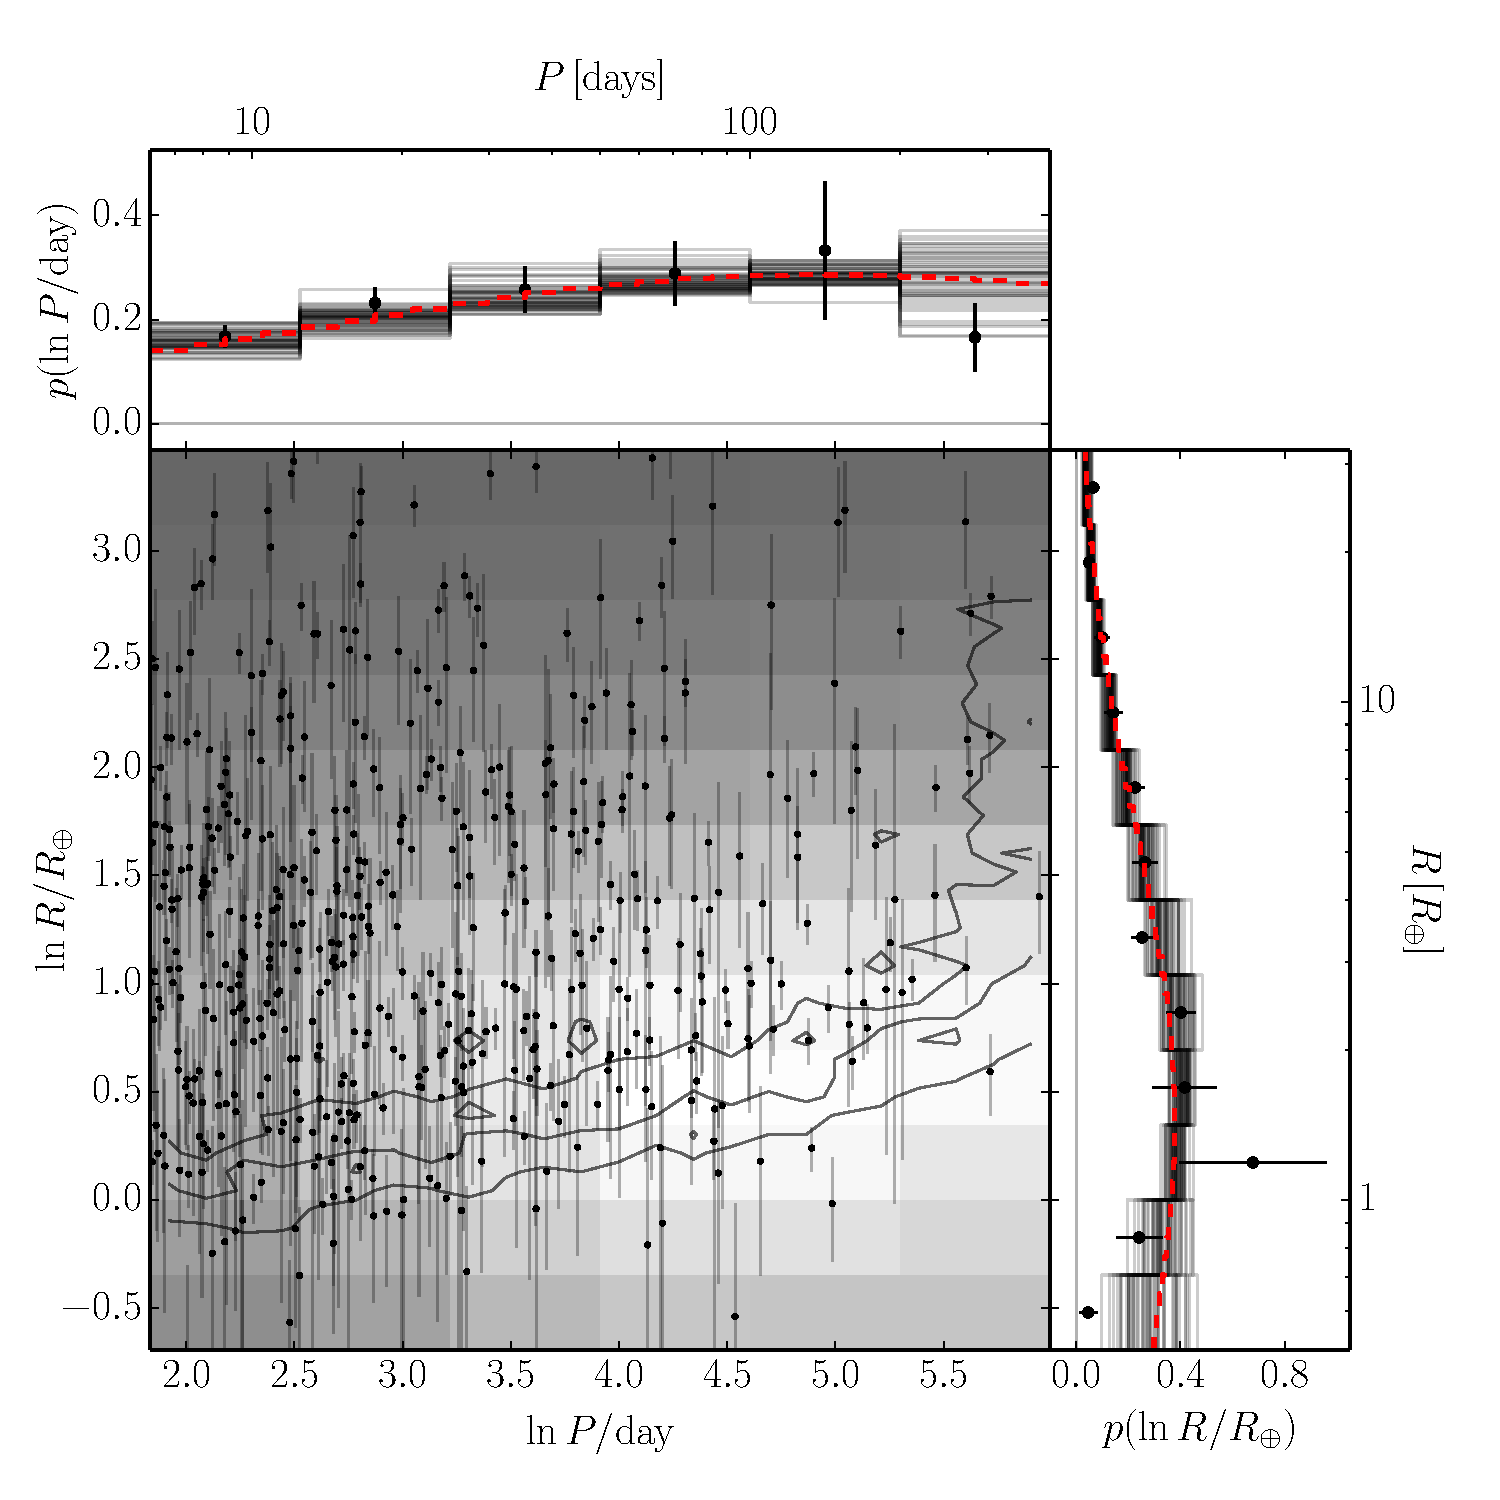
\includegraphics[width=\textwidth]{figures/smooth/results.pdf}
\end{center}
\caption{%
{\bf Simulated data}.
Inferences about the rate density based on the simulated catalog \modela.
\emph{Center:} the points with error bars show the exoplanet candidates in the
simulated incomplete catalog, the contours show the survey completeness
function (\citealt{petigura}), and the grayscale shows the median posterior
occurrence surface.
\emph{Top and left:} the red dashed line shows the true distribution that was
used to generate the catalog, the points with error bars show the results of
the inverse-detection-efficiency procedure, and the histograms are posterior
samples from the marginalized rate density as inferred by our method.
\figlabel{smooth-results}}
\end{figure}

\begin{figure}[p]
\begin{center}
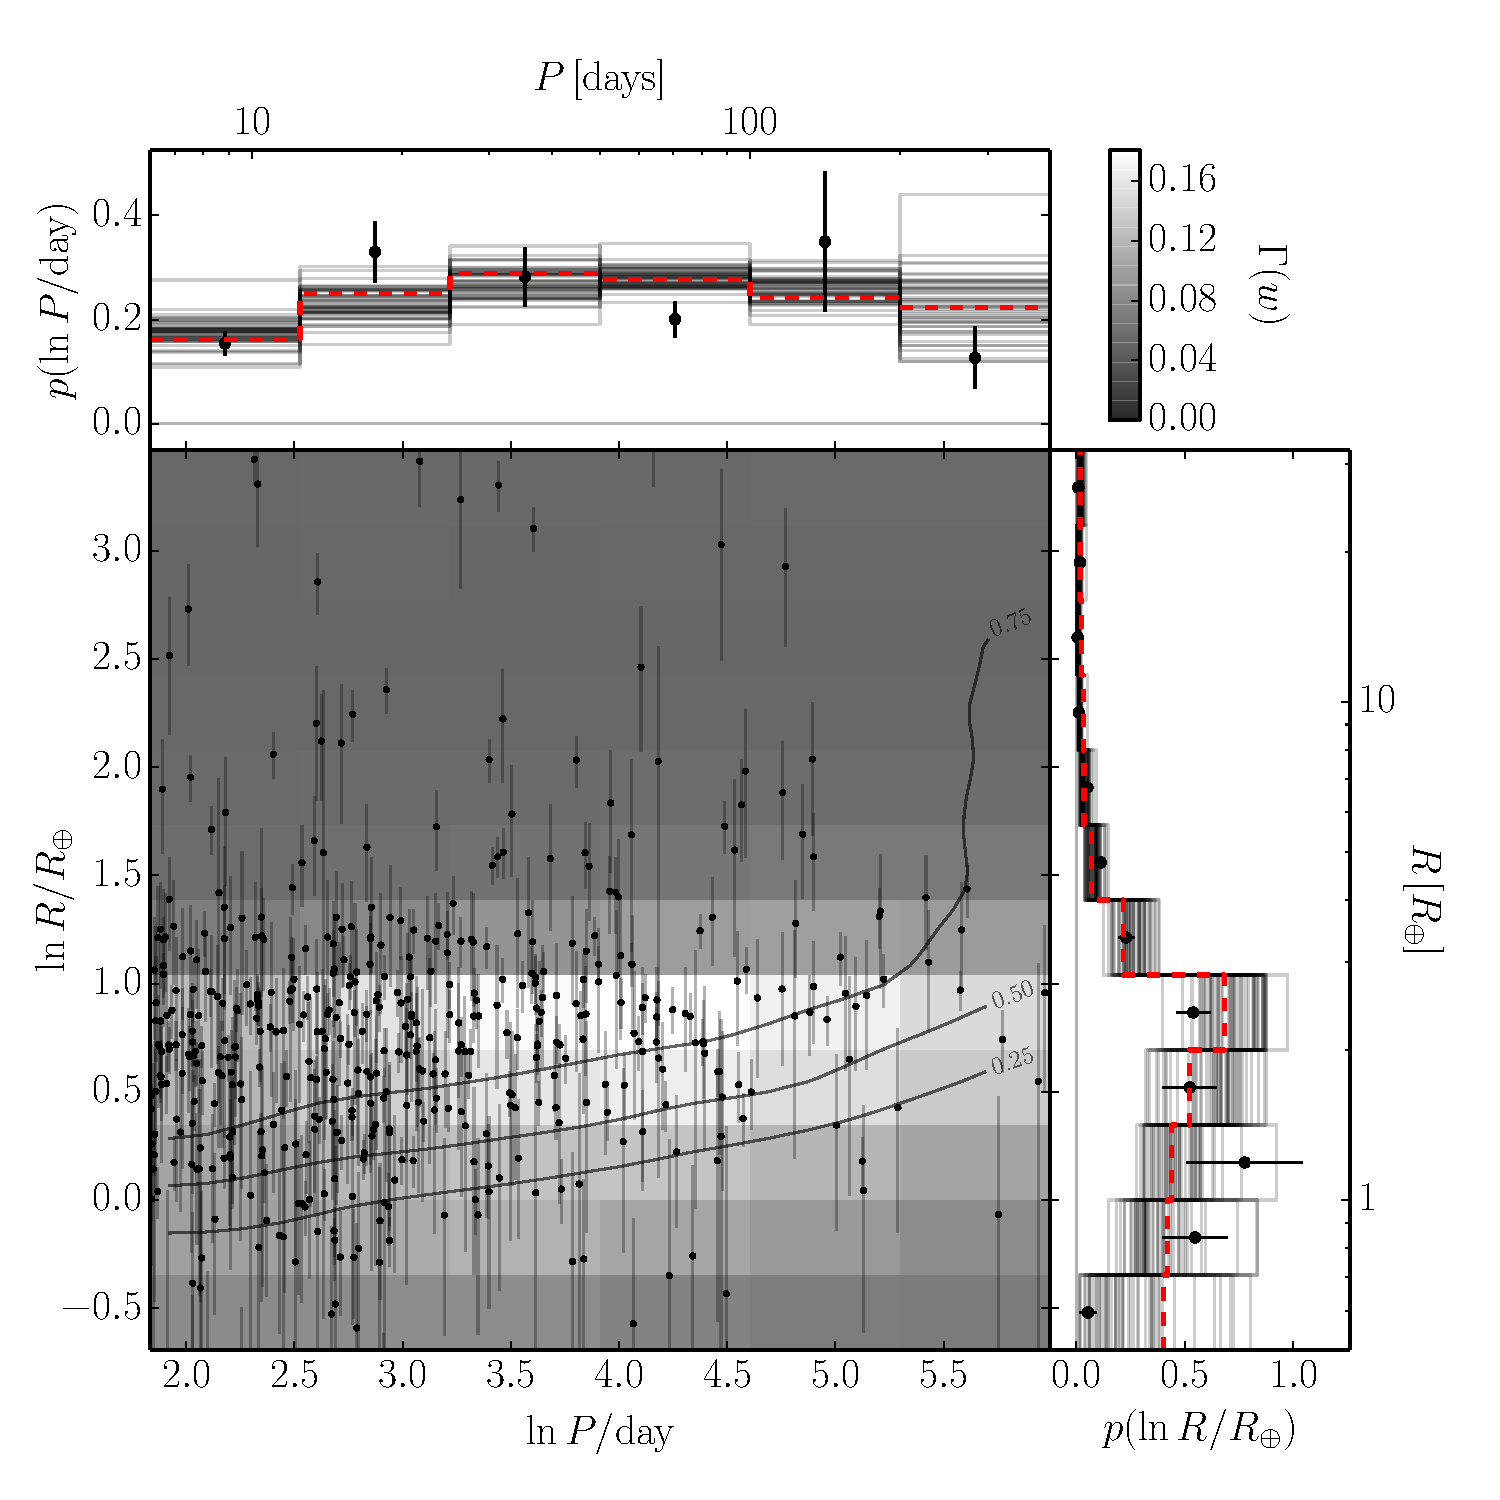
\includegraphics[width=\textwidth]{figures/simulation/results.pdf}
\end{center}
\caption{%
{\bf Simulated data}.
The same as \fig{smooth-results} for \modelb.
\figlabel{simulation-results}}
\end{figure}

\section{Extrapolation to Earth}
\sectlabel{extrap}

As well as inferring the occurrence distribution of exoplanets, this dataset
can also be used to constrain the rate density of Earth analogs.
Explicitly, we constrain the occurrence rate density of exoplanets orbiting
``Sun-like'' stars\footnote{In this \paper, we adopt the \citet{petigura}
sample of G-stars as our definition of ``Sun-like''.}, evaluated at the
location of Earth:
\begin{eqnarray}\eqlabel{gammaearth}
\gammaearth &=& \rate (\ln\period_\oplus,\,\ln\radius_\oplus) \\
&=&
\left.\frac{\dd N}{\dd\ln\period\,\dd\ln\radius}\right|
_{\radius=\radius_\oplus,\,\period=\period_\oplus}\quad.
\end{eqnarray}
That is, \gammaearth\ is the rate density of exoplanets around a Sun-like
star (expected number of planets per star per natural logarithm of period per
natural logarithm of radius), evaluated at the period and radius of Earth.

In \eq{gammaearth}, we define ``Earth analog'' in terms of measurable
quantities with no mention of habitability or composition.
To some readers, this might seem an unsatisfying choice.
That being said, the composition of an exoplanet is notoriously difficult to
measure even with large uncertainty and any definition of habitability is
still extremely subjective.
With this in mind, we stick to the observable definition for this \paper.

Since no Earth analogs have been found, any constraints on this density must
be extrapolated from the existing observations.
This is generally done by assuming a functional form for the occurrence rate
density, constraining it using the observed candidates and extrapolating.
All published extrapolations are based on rigid models of the occurrence rate
density (for example, a power law) fit to the catalog and evaluated at the
location of Earth (\citealt{catanzarite, traub}).
\citet{petigura} used their catalog of planet candidates to constrain the rate
of Earth analogs in a specific period--radius bin assuming an extremely rigid
model: \emph{flat in logarithmic period}.
These results are sensitive to the choice of extrapolation function and the
specific definition of ``Earth analog''.

We weaken the assumptions necessary for extrapolation by only assuming that
the distribution is smooth using the Gaussian process regularization described
in \sect{model}.
Under this model, the occurrence rate density at periods and radii where no
objects have been detected will be constrained---with large uncertainty---by
the heights of nearby bins.
Therefore, even though there are no candidates that qualify as Earth analogs,
we simply fit our model of the occurrence rate density in a large enough
region of parameter space (including Earth) and compute the posterior
constraints on \gammaearth.
This works because the Gaussian process regularization actually captures our
prior beliefs about the shape of the rate density function.
This model---and any other extrapolation---will, of course, break down if
there is an unmeasured sharp feature in the occurrence rate density near the
location of Earth and our method is the most conservative extrapolation
technique published to date.

For comparison, we also implemented and applied the extrapolation technique
applied by \citet{petigura}.
Their method assumes that, for small planets ($1 \le \radius/\radius_\oplus <
2$) on long periods ($\period > 50\,\mathrm{days}$), the occurrence rate
density is a flat function of logarithmic period or, equivalently, the
cumulative rate is linear.
\citet{petigura} used the candidates in their catalog to estimate the slope of
the empirical cumulative period distribution and used that function to
extrapolate.
Instead of defining \gammaearth\ differentially, as we did in \eq{gammaearth},
\citet{petigura} constrained the integral of the rate density over a box in
period and radius ($1 \le \radius/\radius_\oplus < 2$ and $200 \le
\period/\mathrm{day} < 400$).
Since their model implicitly assumes a constant rate density across the bin,
the differential rate is just their number divided by the bin area.
This rate density (rate divided by bin volume) is what is shown as a
comparison to our results in the figures.

Figures~\figref{smooth-rate} and~\figref{simulation-rate} compare our results
and the results of the \citet{petigura} extrapolation procedure when applied
to the synthetic catalogs.
Since these catalogs were simulated from a known population model, we know the
true value of \gammaearth\ and it is indicated in the Figures with a vertical
gray line.
In both cases, our method returns a less precise but more accurate result for
the rate density and the error bars given by the functional extrapolation
are overly optimistic.
One major effect that leads to this bias is that the period distribution is
not flat.
Restricting the result to only include uniform models is equivalent to
applying an extremely informative prior that doesn't have enough freedom to
capture the complexity of the problem.
As a result, the posterior constraints on \gammaearth\ are dominated by this
prior choice and the resulting uncertainties are much smaller than they should
be.

\begin{figure}[p]
\begin{center}
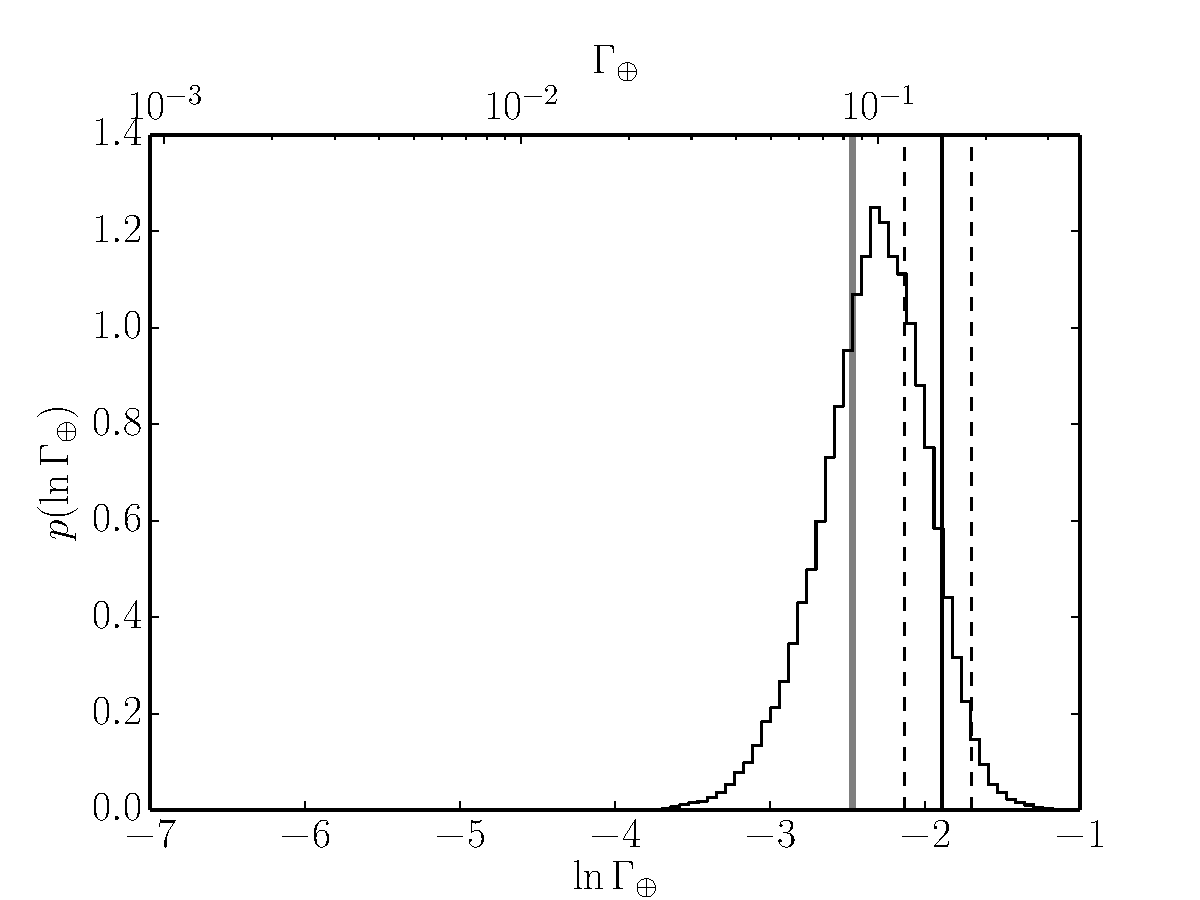
\includegraphics[width=0.6\textwidth]{figures/smooth/rate.pdf}
\end{center}
\caption{%
{\bf Simulated data}.
The extrapolated rate density of Earth analogs \gammaearth\ as inferred by the
different techniques applied to the \modela\ simulation.
Applying the method used by \citet{petigura} gives a constraint indicated by
the vertical black line with error bars shown as dashed lines.
The histogram is the MCMC estimate of our posterior constraint on this rate
density and the true value is indicated as the thick gray vertical line.
\figlabel{smooth-rate}}
\end{figure}

\begin{figure}[p]
\begin{center}
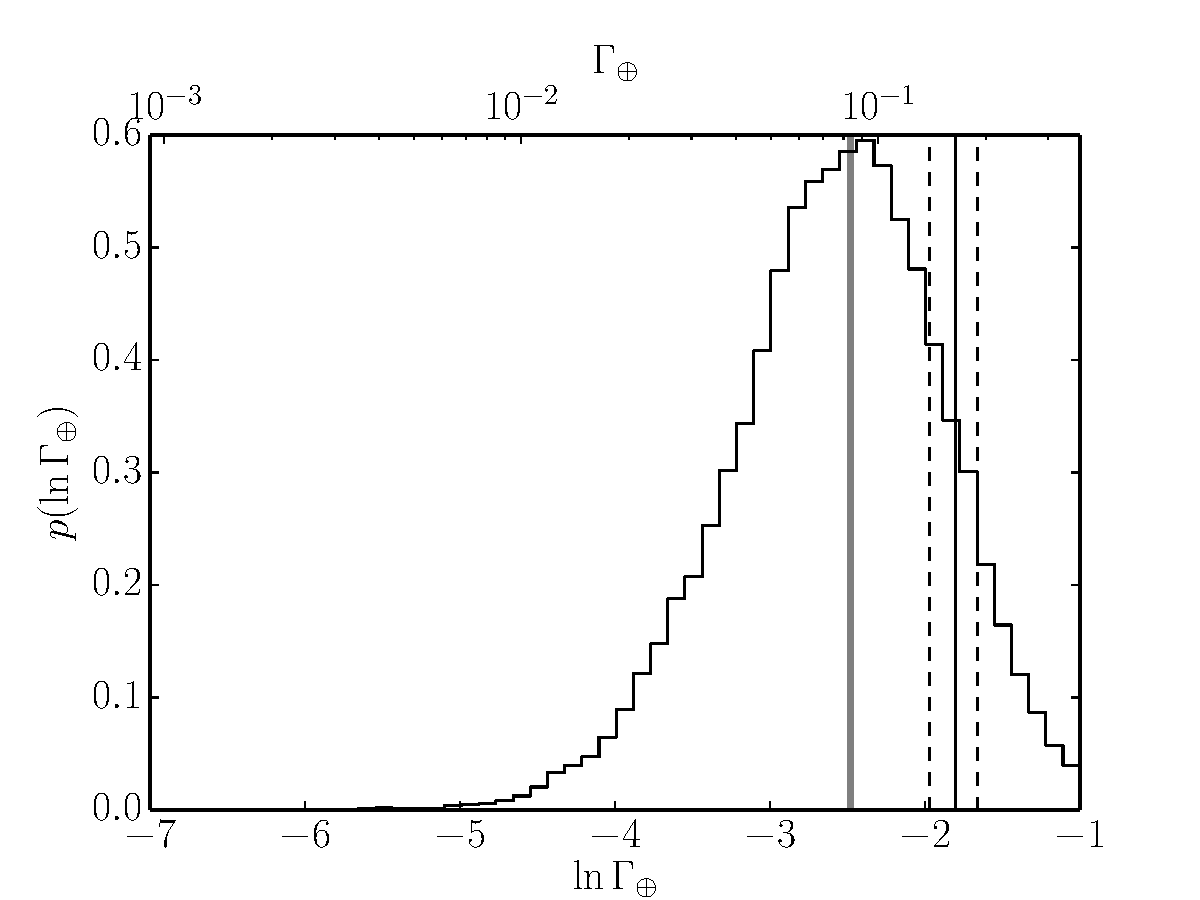
\includegraphics[width=0.6\textwidth]{figures/simulation/rate.pdf}
\end{center}
\caption{%
{\bf Simulated data}.
The same as \fig{smooth-rate} for \modelb.
\figlabel{simulation-rate}}
\end{figure}

\section{Results from real data}

Having developed this probabilistic framework for exoplanet population
inferences and demonstrating that it produces reasonable results when applied
to simulated datasets, we now turn to real data.
As described in \sect{data}, we will use the catalog of small exoplanet
candidates orbiting Sun-like stars published by \citet{petigura}.
This is a great test case because those authors empirically measured the
detection efficiency of their pipeline as a function of the parameters of
interest.

We directly applied our method to the \citet{petigura} sample and generated
MCMC samples from the posterior probability for the occurrence rate density
step heights, marginalizing over the hyperparameters of the Gaussian process
model.
The resulting MCMC chain is available online at \dfmtodo{ADD SOME URL}.

\Fig{real-results} shows posterior samples from the inferred occurrence rate
density as a function of period and radius conditioned on the catalog.
The marginalized distributions are qualitatively consistent with the
occurrence rate density measured using the inverse-detection-efficiency
method with larger uncertainties.

The period distribution integrated over various radius ranges is shown in
\fig{period}.
In agreement with \citet{dong}, we find that the period distribution of large
planets ($R > 8\,R_\oplus$) is inconsistent with the distribution of smaller
planets.
The rate density of large planets appears to monotonically increase as a
function of log period while the distribution for small planets seems to turn
over at a relatively short period (around 50 days) and decrease for larger
periods.

The equivalent Figures for the radius distribution are shown in
Figures~\figref{radius} and~\figref{linear-radius}.
\Fig{radius} shows the log-radius occurrence rate density integrated over
various logarithmic bins in period.
The distributions in each period bin are qualitatively consistent; the
rate density is dominated by small planets (around two Earth radii) with
potential ``features'' near $\radius\sim3\radius_\oplus$ and $\radius\sim
10\radius_\oplus$.
These features appear in every period bin and they were also detected---using
a completely different dataset and technique---by \citet{dong} and a similar
result is visible in the occurrence rate determined by \citet[][their Figure
7]{fressin-fp} at low signal-to-noise.
\Fig{linear-radius} shows the same result but presented as a function of
linear radius.
In these coordinates, the rate density in a single bin is no longer
uniform; instead, scales as inverse radius.

Our constraint on the rate density of Earth analogs (as defined in
\sect{extrap}) is in tension---even though our result has large fractional
uncertainty---with the result from \citet{petigura}.
This is shown in \fig{real-rate} where we compare the marginalized posterior
probability function for \gammaearth\ to the published value and uncertainty.
Quantitatively, we find that the rate density of Earth analogs is
\begin{eqnarray}
\gammaearth &=& 0.017^{+0.018}_{-0.009}~\densityunit
\end{eqnarray}
where the ``\densityunit'' indicates that this quantity is a rate density, per
natural logarithmic period per natural logarithmic radius.
Converted to these units, \citet{petigura} measured
$0.119_{-0.046}^{+0.035}~\densityunit$ for the same quantity (indicated as the
vertical lines in \fig{real-rate}).
This rate density is \emph{exactly} what Petigura's extrapolation model
predicts but, for comparison, we can also integrate our inferred rate density
over their choice of ``Earth-like'' bin ($200 \le \period/\mathrm{day} < 400$
and $1 \le \radius/\radius_\oplus < 2$) to find a \emph{rate} of
Earth-analogs.
The published rate is $0.057_{-0.017}^{+0.022}$ (\citealt{petigura}) and our
posterior constraint is
\begin{eqnarray}
\int_{\period=200\,\mathrm{day}}^{400\,\mathrm{day}}
\int_{\radius=1\,\radius_\oplus}^{2\,\radius_\oplus}
\rate_\ratepars (\ln\period,\,\ln\radius)
\dd[\ln\radius]
\dd[\ln\period]
&=&
0.016_{-0.007}^{+0.011}
\quad.
\end{eqnarray}

\begin{figure}[p]
\begin{center}
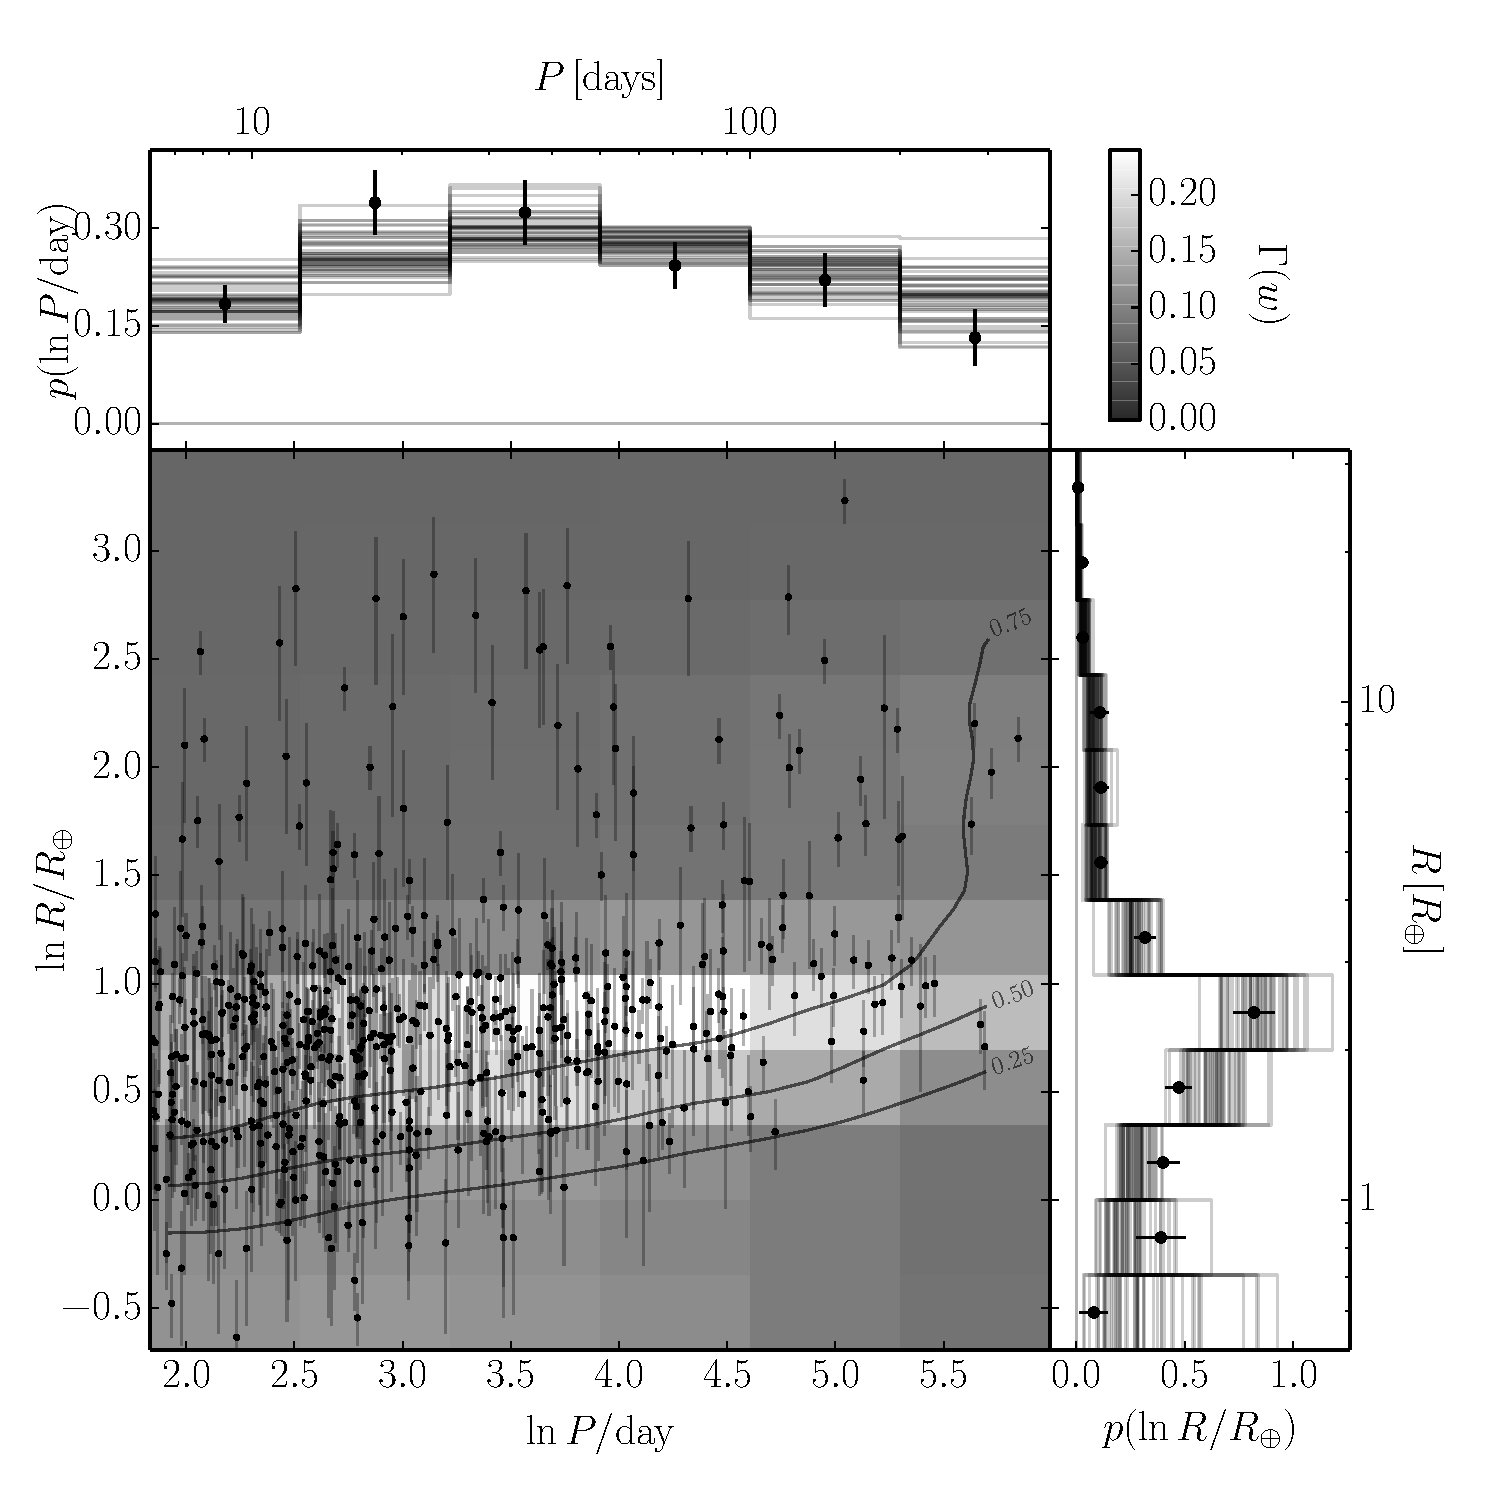
\includegraphics[width=\textwidth]{figures/results/results.pdf}
\end{center}
\caption{%
{\bf Real data}.
The same as \fig{smooth-results} when applied to the observed data from
\citet{petigura}.
\emph{Center:} the points with error bars show the catalog measurements, the
contours show the survey completeness function, and the grayscale shows the
median posterior occurrence surface.
\emph{Top and left:} the points with error bars show the results of the
inverse-detection-efficiency procedure, and the histograms are posterior
samples from the marginalized rate density as inferred by our method.
\figlabel{real-results}}
\end{figure}

\begin{figure}[p]
\begin{center}
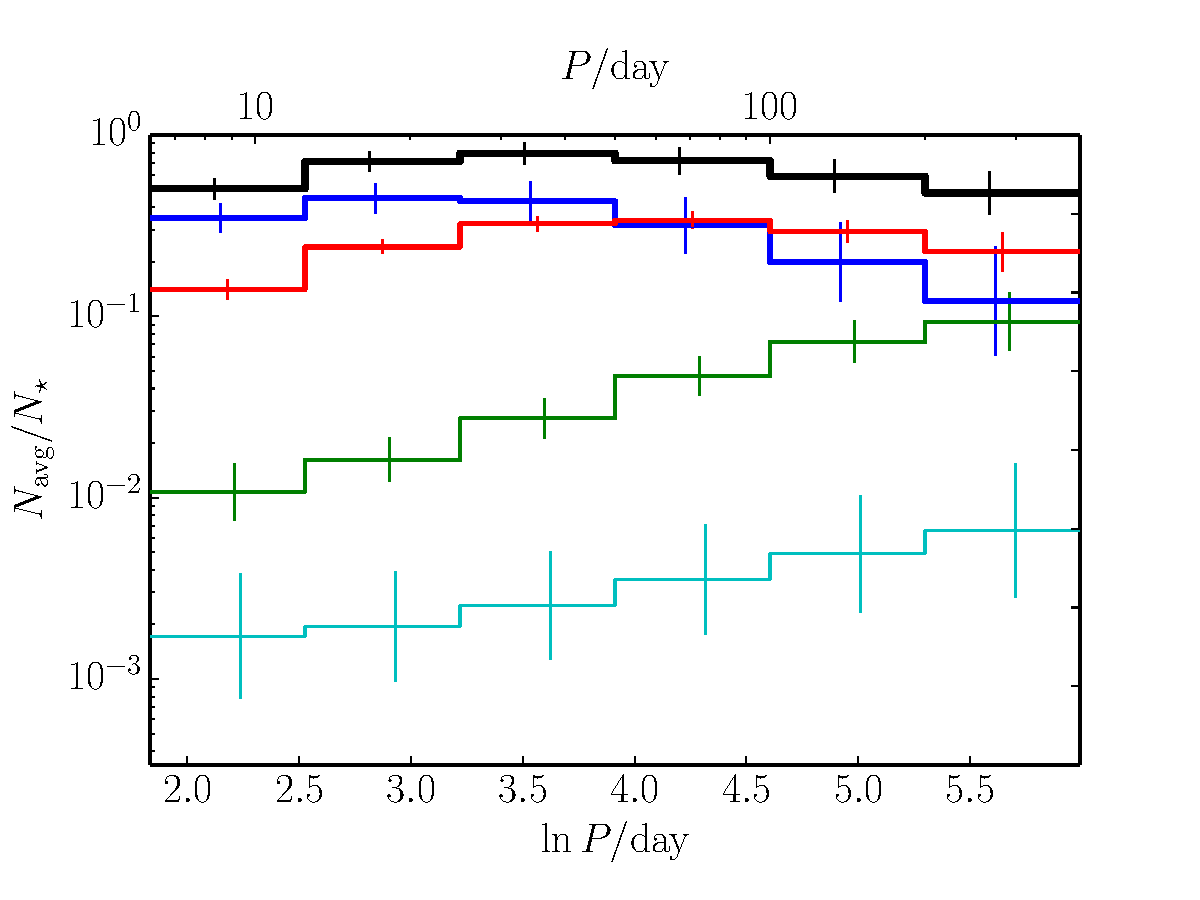
\includegraphics{figures/results/period.pdf}
\end{center}
\caption{%
{\bf Real data}.
The occurrence rate density as a function of logarithmic period integrated
over bins in logarithmic radius.
The lines with error bars show the posterior sample median and 68th
percentile and the line style specifies the radius bin.
The period distribution for the largest planets in the sample
($8 \le R/R_\oplus < 32$) continues to increase (as a function of
$\ln\period$) for all periods while the distribution seems to flatten and
turn over at periods around 50 days.
\figlabel{period}}
\end{figure}

\begin{figure}[p]
\begin{center}
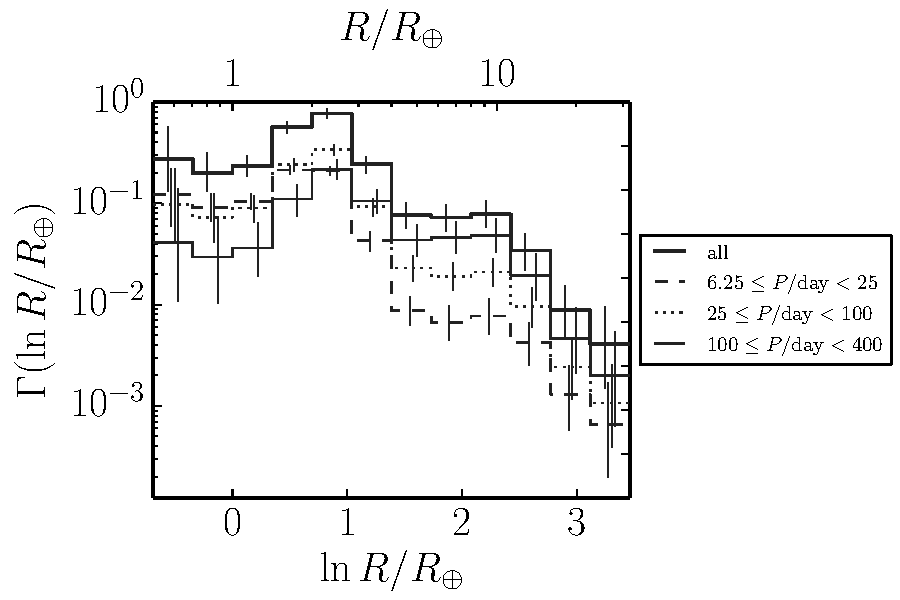
\includegraphics{figures/results/radius.pdf}
\end{center}
\caption{%
{\bf Real data}.
The occurrence rate density as a function of logarithmic radius integrated
over bins in logarithmic period.
The lines with error bars show the posterior sample median and 68th
percentile and the line style specifies the period bin.
The distributions in all the period bins are qualitatively consistent and
there are plausibly features near $R\sim3\,R_\oplus$ and $R\sim10\,R_\oplus$.
\figlabel{radius}}
\end{figure}

\begin{figure}[p]
\begin{center}
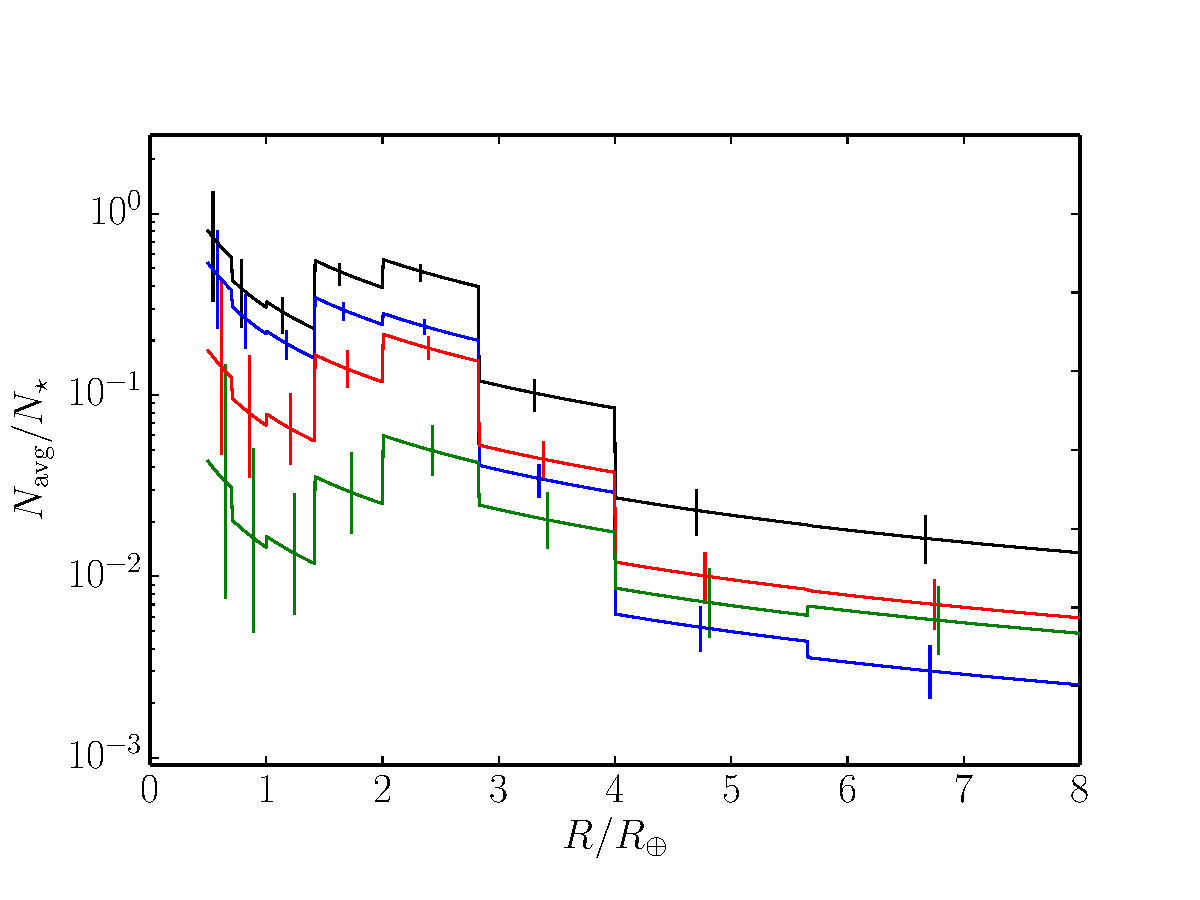
\includegraphics{figures/results/linear-radius.pdf}
\end{center}
\caption{%
{\bf Real data}.
The same as \fig{radius} but presented as a density in radius instead of
logarithmic radius.
\figlabel{linear-radius}}
\end{figure}

\begin{figure}[p]
\begin{center}
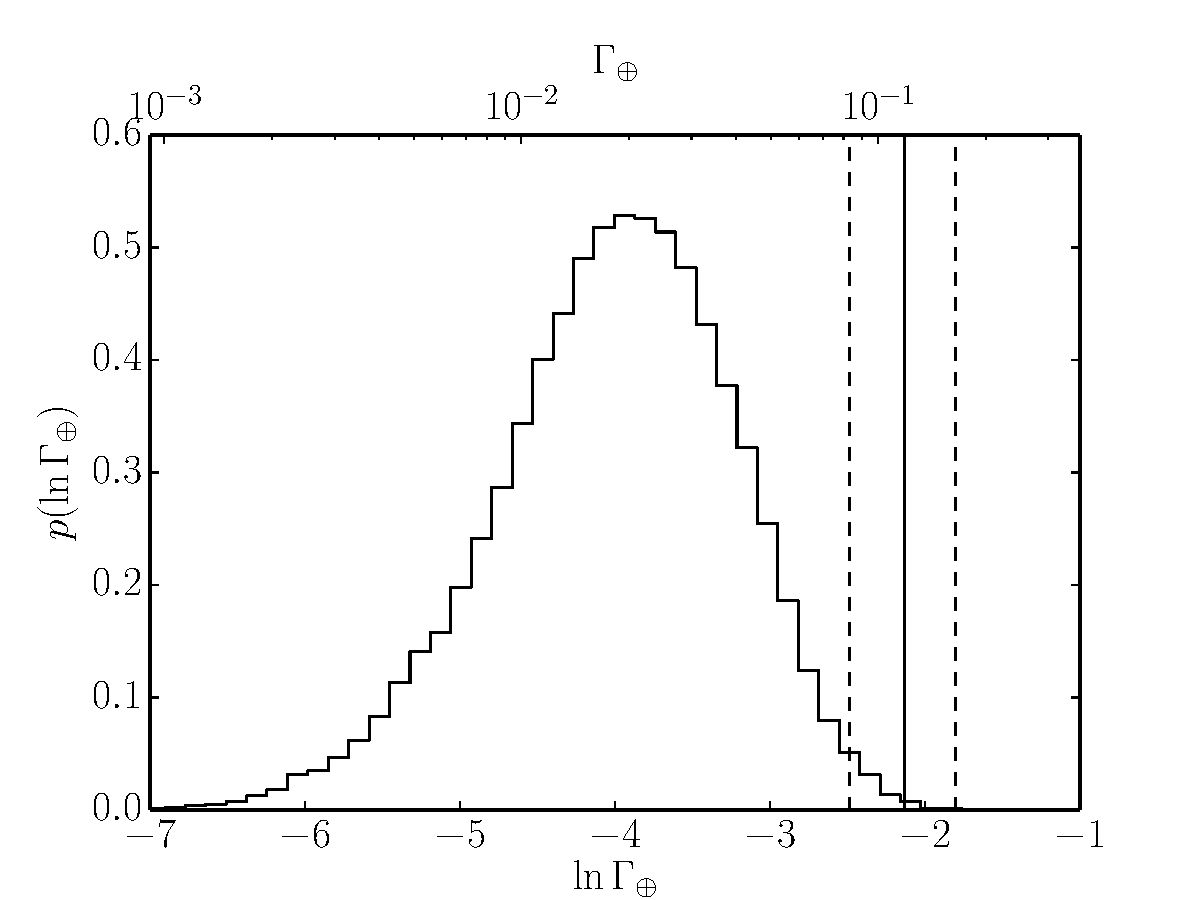
\includegraphics[width=0.6\textwidth]{figures/results/rate.pdf}
\end{center}
\caption{%
The extrapolated rate density of Earth analogs \gammaearth\ (the same as
\fig{smooth-rate} but applied to the catalog from \citealt{petigura}).
The histogram is the MCMC estimate of our posterior constraint on this rate
density.
The vertical black line with error bars shown as dashed lines is the result
from \citet{petigura} converted to a rate density by dividing by their bin
volume.
\figlabel{real-rate}}
\end{figure}

\section{Discussion}

Probabilistic framework justified by MATHS.

Disagrees in detail with Petigura esp.\ extrapolation.

Agrees qualitatively with Petigura, Dong, Howard, \etc\ but hard to make
quantitative comparisons to other ones (pipeline, stars, \etc).

Why did we use the definition of \gammaearth?

Our constraints are less confident---in a signal-to-noise sense---than
previous measurements (made using stronger assumptions; \citealt{petigura})
but, even so, our result is

\dfmtodo{%
Predicted number of observable Earth analogs in the \kepler\ dataset.
Low but not zero.
}

In our analysis we make a few simplifying assumptions.
Each of these could be relaxed and \dfmtodo{BLAH BLAH BLAH}.
\begin{itemize}

\item {\bf Conditional independence}\quad
We assumed that every object in the catalog was a conditionally independent
Poisson draw from the observable occurrence rate function.
This is an interesting assumption to consider when applying this method to a
different catalog where multiple transiting systems are included.
In practice, the best first step towards relaxing this assumption is probably
to follow \citet{tremaine} and assume that the mutual inclination distribution
is the only source of conditional dependence between planets.
For this \paper, the assumption of conditional independence is justified
because the dataset explicitly includes only systems with a single transiting
exoplanet.

\item {\bf False positives}\quad

\item {\bf Known observational uncertainties}\quad

\item {\bf Given empirical detection efficiency}\quad

\item {\bf Smooth rate function}\quad

\end{itemize}

Under these assumptions and the dataset, \etc, we stand by this analysis but
really this is a model of the planets in Kepler convolved with any latent
effects of the TERRA pipeline\ldots

A major effect that isn't taken into account is the highest signal-to-noise
blah blah blah\ldots our number is prolly low.

\dfmtodo{%
{\bf Advice:} \quad
Remind us that we want a representation of the full posterior (samples)
because that would let us do better things with the completeness (modeled as
r/R, \etc).
Must explicitly include priors too.
}


All of the code used in this project is available from
\url{http://github.com/dfm/exopop} under the MIT open-source software license.
This code (plus some dependencies) can be run to re-generate all of the
figures and results in this \paper; this version of the paper was generated
with git commit \texttt{\githash} (\gitdate).

\acknowledgments
We would like to thank Erik Petigura (Berkeley) for freely sharing his data
and code.
It is a pleasure to thank
Ruth Angus (Oxford),
Jo Bovy (IAS), and
Eric Ford (PSU)
for helpful contributions to the ideas and code presented here.
This project was partially supported by the NSF (grant AST-0908357), and NASA
(grant NNX08AJ48G).
This research builds on collaborations between astronomers and statisticians
forged during a three week workshop on ``Modern Statistical and Computational
Methods for Analysis of Kepler Data'' at SAMSI in June 2013.
This research made use of the NASA \project{Astrophysics Data System}.

\newcommand{\arxiv}[1]{\href{http://arxiv.org/abs/#1}{arXiv:#1}}
\begin{thebibliography}{}\raggedright

\bibitem[Adams, Murray \& MacKay(2009)]{poiss-gp}
Adams, R.~P., Murray, I., \& MacKay, D.~J.~C.\ 2009, ICML, 2009, 9
(\href{http://homepages.inf.ed.ac.uk/imurray2/pub/09poisson/}{online})

\bibitem[Ambikasaran \etal(2014)]{dfm-gp}
Ambikasaran, S., Foreman-Mackey, D., Greengard, L., Hogg, D.~W.,
\& O'Neil, M.\ 2014, \arxiv{1403.6015}

\bibitem[Batalha \etal(2013)]{kepler-catalog}
Batalha, N.~M., Rowe, J.~F., Bryson, S.~T., et al.\ 2013, \apjs, 204, 24
(\arxiv{1202.5852})

\bibitem[Brewer \& Stello(2009)]{brewer}
Brewer, B.~J., \& Stello, D.\ 2009, \mnras, 395, 2226 (\arxiv{0902.3907})

\bibitem[Carter \& Winn(2009)]{carter}
Carter, J.~A., \& Winn, J.~N.\ 2009, \apj, 704, 51 (\arxiv{0909.0747})

\bibitem[Catanzarite \& Shao(2011)]{catanzarite}
Catanzarite, J., \& Shao, M.\ 2011, \apj, 738, 151 (\arxiv{1103.1443})

\bibitem[Dong \& Zhu(2013)]{dong}
Dong, S., \& Zhu, Z.\ 2013, \apj, 778, 53 (\arxiv{1212.4853})

\bibitem[Dressing  \& Charbonneau(2013)]{dressing}
Dressing, C.~D., \& Charbonneau, D.\ 2013, \apj, 767, 95 (\arxiv{1302.1647})

\bibitem[Fang \& Margot(2012)]{fang}
Fang, J., \& Margot, J.-L.\ 2012, \apj, 761, 92 (\arxiv{1207.5250})

\bibitem[Foreman-Mackey \etal(2012)]{emcee}
Foreman-Mackey, D., Hogg, D.~W., Lang, D., \& Goodman, J.\ 2013, \pasp, 125,
306 (\arxiv{1202.3665})

\bibitem[Fressin \etal(2013)]{fressin-fp}
Fressin, F., Torres, G., Charbonneau, D., \etal\ 2013, \apj, 766, 81
(\arxiv{1301.0842})

\bibitem[Gibson \etal(2012)]{gibson-gp}
Gibson, N.~P., Aigrain, S., Roberts, S., \etal\ 2012, \mnras, 419, 2683
(\arxiv{1109.3251})

\bibitem[Hogg \etal(2013)]{hoggwhitepaper}
Hogg, D.~W., Angus, R., Barclay, T., et al.\ 2013, \arxiv{1309.0653}

\bibitem[Hogg \etal(2010)]{hogge}
Hogg, D.~W., Myers, A.~D., \& Bovy, J.\ 2010, \apj, 725, 2166
(\arxiv{1008.4146})

\bibitem[Howard \etal(2012)]{howard}
Howard, A.~W., Marcy, G.~W., Bryson, S.~T., et al.\ 2012, \apjs, 201, 15
(\arxiv{1103.2541})

\bibitem[Lewis \& Shedler(1979)]{poisson}
Lewis, P.~A.~W., \& Shedler, G.~S.\ 1979, Naval Research Logistics Quarterly,
26, 403

\bibitem[Lissauer \etal(2011)]{lissauer}
Lissauer, J.~J., Ragozzine, D., Fabrycky, D.~C., et al.\ 2011, \apjs, 197, 8
(\arxiv{1102.0543})

\bibitem[Morton \& Johnson(2011)]{morton}
Morton, T.~D., \& Johnson, J.~A.\ 2011, \apj, 738, 170 (\arxiv{1101.5630})

\bibitem[Morton \& Swift(2013)]{morton-swift}
Morton, T.~D., \& Swift, J.~J.\ 2013, \arxiv{1303.3013}

\bibitem[Murray \etal(2010)]{ess}
Murray, I., Prescott Adams, R., \& MacKay, D.~J.~C.\ 2010, JMLR: W\&CP, 9, 541
(\arxiv{1001.0175})

\bibitem[Murray \& Prescott Adams(2010)]{ess-hyper}
Murray, I., \& Prescott Adams, R.\ 2010, Advances in Neural Information
Processing Systems, 23, 1723
(\arxiv{1006.0868})

\bibitem[Petigura \etal(2013a)]{petigura-a}
Petigura, E.~A., Marcy, G.~W., \& Howard, A.~W.\ 2013a, \apj, 770, 69
(\arxiv{1304.0460})

\bibitem[Petigura \etal(2013b)]{petigura}
Petigura, E.~A., Howard, A.~W., \& Marcy, G.~W.\ 2013b,
Proceedings of the National Academy of Science, 110, 19273 (\arxiv{1311.6806})

\bibitem[Rasmussen \& Williams(2006)]{gp}
Rasmussen, C.~E. \& Williams, C.~K.~I.\ 2006
Gaussian Processes for Machine Learning, MIT Press
(\href{http://www.gaussianprocess.org/gpml/}{online})

\bibitem[Roberts \etal(2013)]{roberts}
Roberts, S., McQuillan, A., Reece, S., \& Aigrain, S.\ 2013, \mnras, 435, 3639
(\arxiv{1308.3644})

\bibitem[Swift \etal(2013)]{swift}
Swift, J.~J., Johnson, J.~A., Morton, T.~D., et al.\ 2013, \apj, 764, 105
(\arxiv{1301.0023})

\bibitem[Tabachnik \& Tremaine(2002)]{tabachnik}
Tabachnik, S., \& Tremaine, S.\ 2002, \mnras, 335, 151
(\arxiv{astro-ph/0107482})

\bibitem[Traub(2012)]{traub}
Traub, W.~A.\ 2012, \apj, 745, 20 (\arxiv{1109.4682})

\bibitem[Tremaine \& Dong(2012)]{tremaine}
Tremaine, S., \& Dong, S.\ 2012, \aj, 143, 94 (\arxiv{1106.5403})

\bibitem[Youdin(2011)]{youdin}
Youdin, A.~N.\ 2011, \apj, 742, 38 (\arxiv{1105.1782})

\end{thebibliography}

\end{document}
